\documentclass[../../main.tex]{subfiles}
\begin{document}

{\bf [解]}
$A(1,0)$ ，$|AP|$ の中点 $M_1$ とする．
$\angle M_1OA=\theta$ とすると，下図より$|OA|$ から $|OQ|$ へ向かう角は $4\theta$ であるから，
\begin{align}
 Q(\cos4\theta,\sin4\theta) \label{eq:1}
\end{align}
となる．

\begin{figure}[htb]
\begin{center}
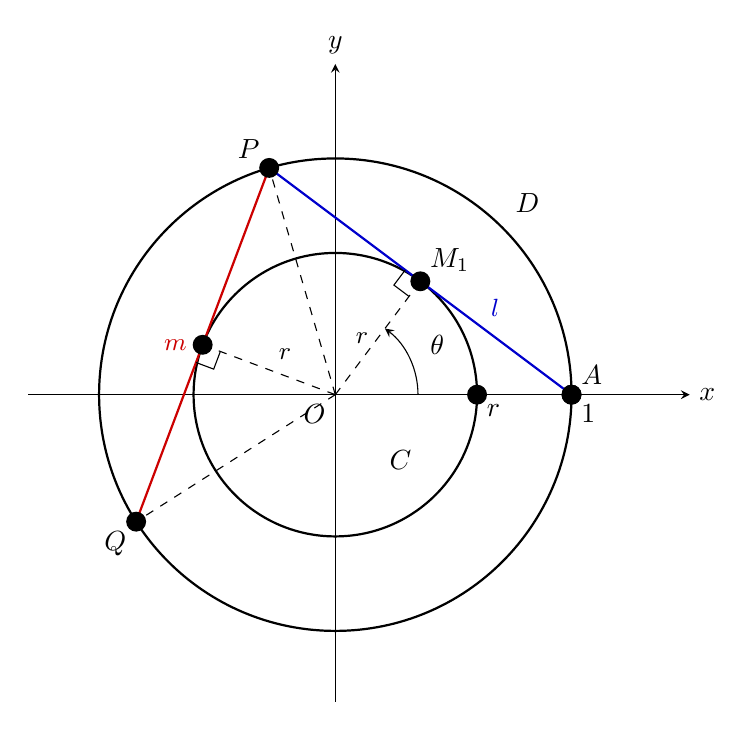
\begin{tikzpicture}[scale=3, >=stealth]
  % パラメータ設定 (r = cos(theta) = 0.6 とする)
  \def\r{0.6}
  \def\thetaVal{53.13} % cos(53.13°) = 0.6

  % 1. 座標軸
  \draw[->] (-1.3, 0) -- (1.5, 0) node[right] {$x$};
  \draw[->] (0, -1.3) -- (0, 1.4) node[above] {$y$};
  \node[below left] at (0,0) {$O$};

  % 2. 円 C (半径 r) と 円 D (半径 1)
  \draw[thick] (0,0) circle (\r);
  \node at (-45:{\r*0.65}) {$C$};
  \draw[thick] (0,0) circle (1);
  \node at (45:1.15) {$D$};

  % 3. 主要な点の座標
  \coordinate (A)  at (1,0);                                       % A(1,0) [M_1]
  \coordinate (C1) at ({\r*cos(\thetaVal)}, {\r*sin(\thetaVal)}); % l と C の接点
  \coordinate (P)  at ({cos(2*\thetaVal)}, {sin(2*\thetaVal)});   % 点 P (角度 2theta)
  \coordinate (C2) at ({\r*cos(3*\thetaVal)}, {\r*sin(3*\thetaVal)}); % m と C の接点
  \coordinate (Q)  at ({cos(4*\thetaVal)}, {sin(4*\thetaVal)});   % 点 Q (角度 4theta)

  % 4. 接線 l と 接线 m の描画
  % 接線 l ( (1,0) から P へ )
  \draw[thick, blue!80!black] (A) -- (P) node[pos=0.3, above right, font=\small] {$l$};
  % 接線 m ( P から Q へ )
  \draw[thick, red!80!black] (P) -- (Q) node[midway, left=2pt, font=\small] {$m$};

  % 5. 補助線（接点への垂線・動径）
  \draw[dashed] (0,0) -- (C1) node[midway, left, font=\small] {$r$};
  \draw[dashed] (0,0) -- (C2) node[midway, above right, font=\small] {$r$};
  \draw[dashed] (0,0) -- (P);
  \draw[dashed] (0,0) -- (Q);

  % 接点における直角マーク
  \begin{scope}[rotate=\thetaVal]
    \draw (\r-0.08, 0) -- (\r-0.08, 0.08) -- (\r, 0.08);
  \end{scope}
  \begin{scope}[rotate=3*\thetaVal]
    \draw (\r-0.08, 0) -- (\r-0.08, 0.08) -- (\r, 0.08);
  \end{scope}

  % 6. 点のプロットとラベル
  \fill (A)  circle (1.2pt) node[below right] {$1$};
  \fill (A)  circle (1.2pt) node[above right] {$A$};
  \fill (\r,0)  circle (1.2pt) node[below right] {$r$};
  \fill (C1) circle (1.2pt) node[above right] {$M_1$};
  \fill (P)  circle (1.2pt) node[above left] {$P$};
  \fill (C2) circle (1.2pt);
  \fill (Q)  circle (1.2pt) node[below left] {$Q$};

  % 7. 角度 theta の表示
  \draw[->] (0.35,0) arc (0:\thetaVal:0.35);
  \node at (26:0.48) {$\theta$};

\end{tikzpicture}
\end{center}
\caption{問題の状況と点 $P, Q$ の位置関係}
\end{figure}


\begin{figure}[htb]
\begin{center}
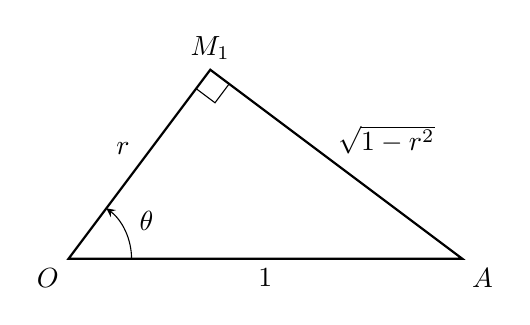
\begin{tikzpicture}[scale=2, >=stealth]
  % パラメータ設定 (cos(theta) = r = 0.6)
  \def\r{0.6}
  \def\thetaVal{53.13} % cos(53.13°) ≒ 0.6

  % 頂点の定義
  \coordinate (O)  at (0, 0);
  \coordinate (A)  at (2.5, 0); % 斜辺 OA の長さ
  \coordinate (M1) at ({\r*2.5*cos(\thetaVal)}, {\r*2.5*sin(\thetaVal)}); % 頂点 M_1

  % 三角形 M_1OA の描画
  \draw[thick] (O) -- (A) -- (M1) -- cycle;

  % 直角マーク (M_1 における垂直記号)
  \begin{scope}[shift={(M1)}, rotate={\thetaVal - 90}]
    \draw (0.15,0) -- (0.15, -0.15) -- (0, -0.15);
  \end{scope}

  % 角 theta の表示
  \draw[->] (0.4, 0) arc (0:\thetaVal:0.4);
  \node at (26:0.55) {$\theta$};

  % 各辺の長さのラベル
  \node[above left] at (0.45, 0.6) {$r$};
  \node[above right] at (1.65, 0.6) {$\sqrt{1-r^2}$};
  \node[below] at (1.25, 0) {$1$};

  % 頂点ラベル
  \node[below left] at (O) {$O$};
  \node[below right] at (A) {$A$};
  \node[above] at (M1) {$M_1$};

\end{tikzpicture}
\end{center}
\caption{直角三角形 $\triangle M_1OA$}
\end{figure}

ここで上図の三角形 $\triangle M_1OA$ に注目して，
\begin{align}
\sin\theta=\sqrt{1-r^2}, \quad \cos\theta=r \label{eq:2}
\end{align}
だから，倍角公式を繰り返し用いて
\begin{align}
\cos4\theta
   &=2\cos^22\theta-1 \\
   &=2(2\cos^2\theta-1)^2-1 \\
   &=2(2r^2-1)^2-1 \quad (\because \cref{eq:2} ) \\
   &= 8r^4-8r^2+1
\end{align}
および
\begin{align}
\sin4\theta
   &=2\sin2\theta\cos2\theta \\
   &=4\sin\theta\cos\theta\cdot(2\cos^2\theta-1) \\
   &=4r\sqrt{1-r^2}(2r^2-1) \quad (\because \cref{eq:2} )
\end{align}
となる．これらを\cref{eq:1}に代入して求める$Q$の座標は
\begin{align}
Q\left(8r^4-8r^2+1,\ 4r(2r^2-1)\sqrt{1-r^2}\right)
\end{align}
である．


\newpage

\end{document}
